\chapter{Evaluation}
The following Chapter provides an overview of distribution scenarios and the efficiency of the in this theses developed tool. The table \ref{tab:devices} shows the different devices that are employed during the evaluation process. Patricks-MBP is located in one WIFI network. Fioo.one is located at a different place and in a different WIFI network. The AWS instances are publicly accessible.


\begin{table}[h]
\begin{center}
    \begin{tabular}{ | m{5em} | m{5em}| m{6em} | m{5em} | m{5em}| m{6em} | }
      \hline
      Name & Device & Processor & Memory & OS & Architecture \\ 
      \hline
      Patricks-MBP & MacBook Pro (15-inch, 2017) & 4 x 2.8 GHz & 16 GB & macOS Big Sur & amd64 \\
      \hline
      fioo.one & AMD Ryzen 5 4500U & 6 x 2.3 GHz & 16 GB & Ubuntu 21.04 & amd64 \\
      \hline
      AWS EC2 instances & C4.8xlarge & 36 x vCPU 2.9 GHz Intel Xeon E5-2666 v3 Processor & 60 GB & Amazon Linux & amd64 \\
      \hline
    \end{tabular}
    \caption{\label{tab:devices} Test devices}
\end{center}
\end{table}

\section{Scenarios}

Each scenario is run 5 times to average the results. The used simulation is the “tictoc” example that comes with OMNeT++. The executed configuration is “TicToc18”, because it runs various parameter combinations which can be dispersed. The benchmark scenarios can be found in Table \ref{tab:benchmarks}. The different scenarios, that use the tools developed in this work, are manifested in Table \ref{tab:scenarios}.


\begin{table}[h]
\begin{center}
    \begin{tabular}{ | m{6em} | m{16em}| m{12em} | }
      \hline
      Scenario & Worker & Number of parallel Jobs \\ 
      \hline
      opp-run-j1 & Patricks-MBP & 1 \\
      \hline
      opp-run-j2 & Patricks-MBP & 2 \\
      \hline
      opp-run-j4 & Patricks-MBP & 4 \\
      \hline
    \end{tabular}
    \caption{\label{tab:benchmarks} Benchmark scenarios}
\end{center}
\end{table}


\begin{table}[h]
\begin{center}
    \begin{tabular}{ | m{8em} | m{5em}| m{4em} | m{6em} | m{6em}| m{3em} | }
      \hline
      Scenario & Worker & Parallel Jobs & Started from & Connection & Docker \\ 
      \hline
      MacBook-j1 & Patricks-MBP & 1 & Patricks-MBP & Local (loop-back) & FALSE \\
      \hline
      MacBook-j2 & Patricks-MBP & 2 & Patricks-MBP & Local (loop-back) & FALSE \\
      \hline
      MacBook-j4 & Patricks-MBP & 4 & Patricks-MBP & Local (loop-back) & FALSE \\
      \hline
      MacBook-j1-p2p & Patricks-MBP & 1 & fioo.one & Peer-to-peer & FALSE \\
      \hline
      MacBook-j4-p2p & Patricks-MBP & 4 & fioo.one & Peer-to-peer & FALSE \\
      \hline
      MacBook-j1-relay & Patricks-MBP & 1 & fioo.one & Relay server & FALSE \\
      \hline
      MacBook-j4-relay & Patricks-MBP & 4 & fioo.one & Relay server & FALSE \\
      \hline
      MacBook-j1-p2p-docker & Patricks-MBP & 1 & fioo.one & Peer-to-peer & TRUE \\
      \hline
      AWS-j32 & c4.8xlarge & 32 & Patricks-MBP & Peer-to-peer & TRUE \\
      \hline
      AWS-j62 & c4.8xlarge, c4.8xlarge & 64 & Patricks-MBP & Peer-to-peer & TRUE \\
      \hline
    \end{tabular}
    \caption{\label{tab:scenarios} Evaluation scenarios}
\end{center}
\end{table}

\section{Benchmark Scenario}

Scenario opp-run-j1, opp-run-j2, and opp-run-j4 are the benchmark scenarios. The scenarios are executed locally with “opp\_runall”. Scenario opp-run-j1 is executed single threaded, opp-run-j2 is executed with two parallel jobs, and opp-run-j4 is executed with four parallel jobs. Figure ~\ref{fig:eval-benchmark} shows the average execution duration time for these three scenarios.

\begin{figure}[h]
  \centering
  \includesvg[width=250pt]{images/eval/benchmark/Mean execution duration per simulation.svg}
  \caption{Benchmark: Mean execution duration per simulation}
  \label{fig:eval-benchmark}
\end{figure}

The benchmarks can be compared to execution times that use the tool developed by this thesis to measure how much overhead is added by the distribution and offloading process. The results can be viewed in Figure \ref{fig:eval-overhead}. The scenarios will use the same number of CPU cores to display parallelizing effects. Scenario clj1is only located on Patricks-MBP and runs with opp\_edge\_run and one worker that uses one CPU core. Opp-run-j1 needs 154 seconds for execution. Clj1 needs 192 seconds. The distribution process adds an overhead of 38 seconds to the simulation. When the scenario runs with four simulation jobs, the native version needs 48 seconds, and the distributed version needs 69 seconds. The overhead is 21 seconds. The concurrent version has less overhead than the distributed version because the download process happens faster because there is less delay for the downloader between finished jobs. 
\begin{figure}[h]
  \centering
  %\includesvg[width=250pt]{images/eval/overhead/Mean execution duration per simulation.svg}
  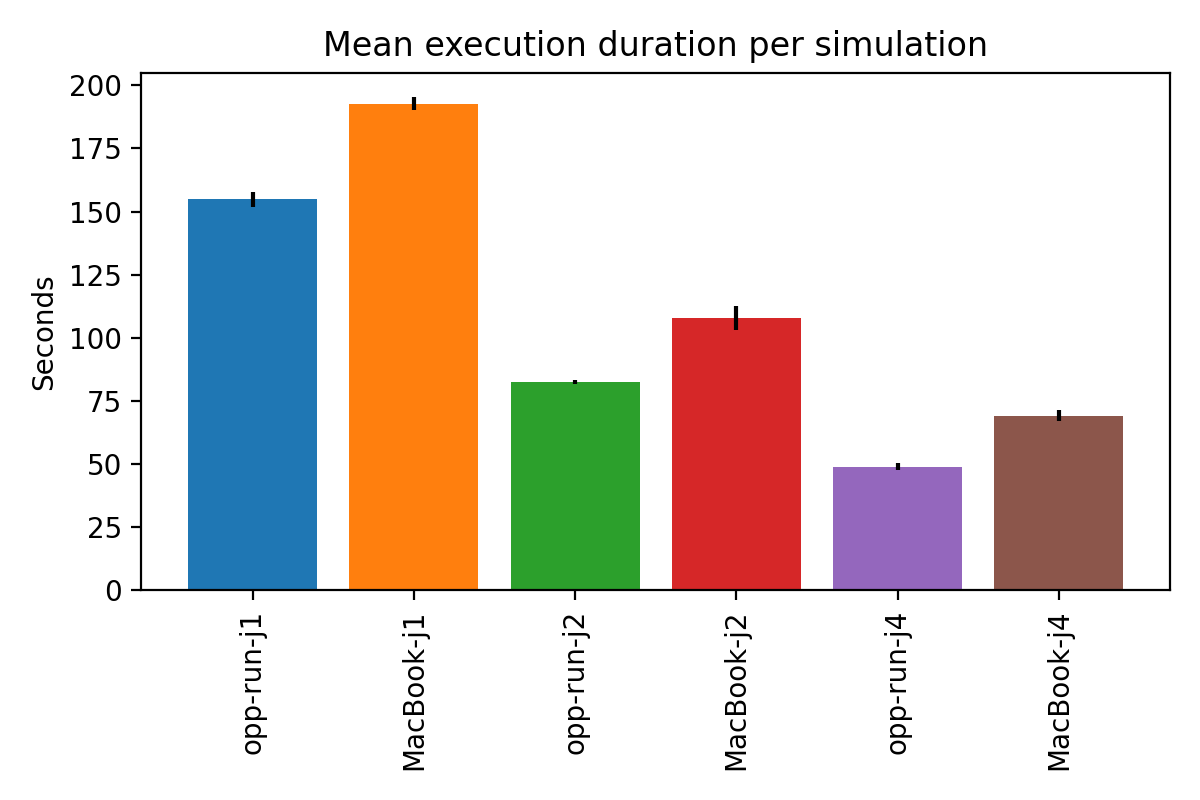
\includegraphics[width=250pt]{images/eval/overhead/Mean execution duration per simulation}
  \caption{Overhead: Mean execution duration per simulation}
  \label{fig:eval-overhead}
\end{figure}

Figure ~\ref{fig:eval-overhead-run} shows the average execution time per simulation-run. Scenario “clj4” has a slightly slower execution time because it is subject to thermal throttling effects. 

\begin{figure}[h]
  \centering
  \includesvg[width=250pt]{images/eval/overhead/Mean execution duration per simulation-run.svg}
  \caption{Overhead: Mean execution duration per simulation run}
  \label{fig:eval-overhead-run}
\end{figure}





\section{Connection overhead}

Providers and consumers connect over three ways: over a TCP connection in the local network, over a peer-to-peer UDP connection or over a TCP connection over a relay server. These connections can have different transfer rates which influence how fast simulation results can be transferred between the consumer and providers. Slow transfer rates are a bottleneck.

The local connection should be fastest, because the traffic doesn't leave the local network. The peer-to-peer connection should be second because it leaves the local network but is sent to the peer directly. The slowest should be the relay connection because the traffic is relayed by a central point. Figure ~\ref{fig:eval-connect-transfer} shows the download and upload transfer rates. The difference between the peer-to-peer and relay rates are neglectable, but it should be noted that at the time of the experiment no other client used the relay connection at the server. The peer-to-peer connection is preferred because it reduces traffic at the broker and is less susceptible.

\begin{figure}[h]
  \centering
  \includesvg[width=250pt]{images/eval/connect/Transfer Rate.svg}
  \caption{Connect: Transfer rates for the three connection ways}
  \label{fig:eval-connect-transfer}
\end{figure}

\section{Docker overhead}

For convenience and security reasons the provider software can be started from a Docker container. The Docker virtualization adds some overhead that can be seen in Figure \ref{fig:eval-docker-sim-run}. The measured overhead is approximately 15\%.

\begin{figure}[h]
  \centering
  %\includesvg[width=250pt]{images/eval/docker/Mean execution duration per simulation.svg}
  
\includegraphics[width=250pt]{images/eval/docker/Mean execution duration per simulation}
  \caption{Docker: Mean execution duration per simulation}
  \label{fig:eval-docker-sim-run}
\end{figure}




\section{Maximal Parallelization}

The Figure \ref{fig:eval-aws-duration} shows the effect of nearly complete parallelization. The “tictoc” simulation example has a total of 78 simulation-runs. The scenario “cp.aws.c48xlarge.x2” has a total of 64 CPUs that can start 64 simulation-runs in parallel. The data shows that a simulation which is executed with one CPU core needs a total of 184 seconds. A simulation that is executed with 64 CPU cores just needs 18 seconds, which is a speed up of approximately 10 times.

\begin{figure}[h]
  \centering
  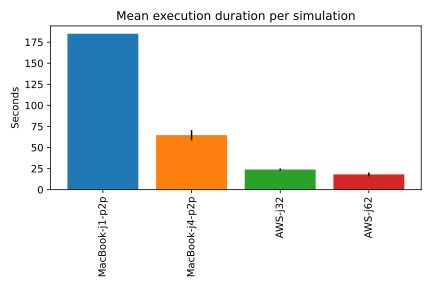
\includegraphics[width=250pt]{images/eval/aws/Mean execution duration per simulation}
  \caption{AWS: Mean execution duration per simulation}
  \label{fig:eval-aws-duration}
\end{figure}

Figure \ref{fig:eval-aws-transfer} shows that the download and upload transfer rates are approximately the same.

\begin{figure}[h]
  \centering
  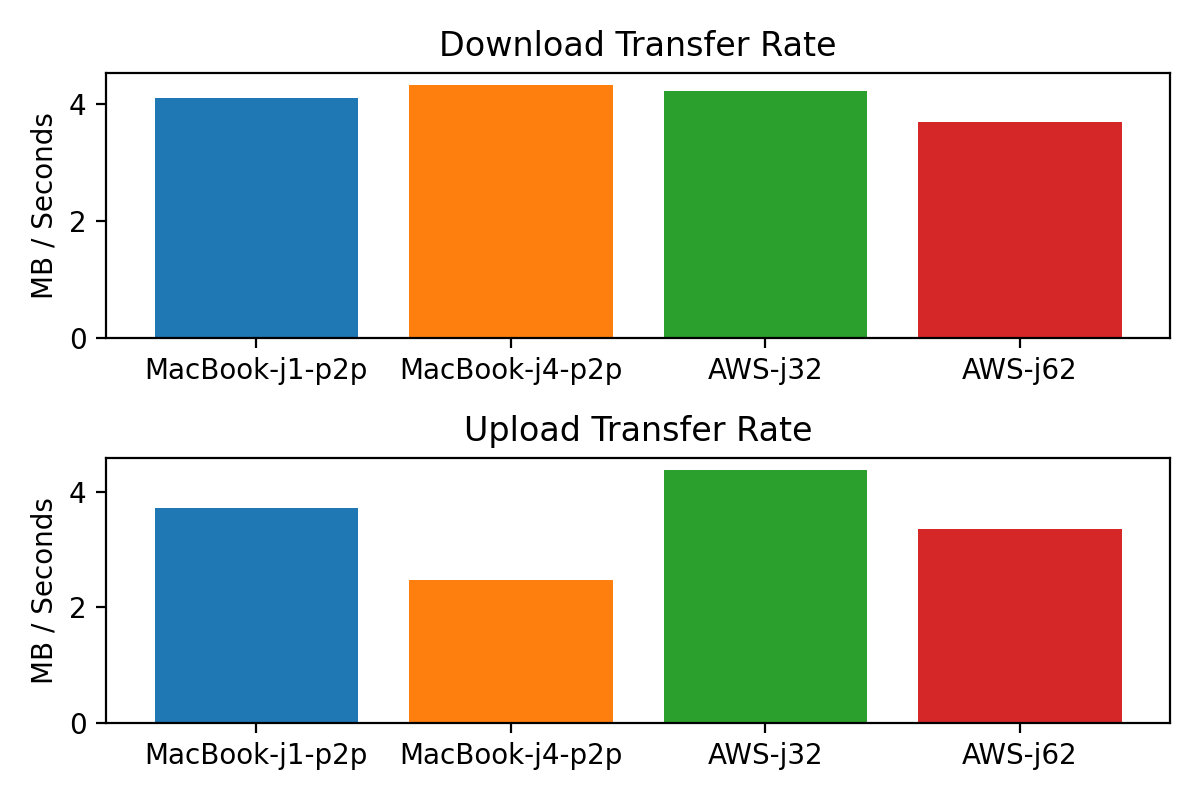
\includegraphics[width=250pt]{images/eval/aws/Transfer Rate}
  \caption{AWS: Transfer rates for the scenarios}
  \label{fig:eval-aws-transfer}
\end{figure}
